% Chapter 5: Project planning

\chapter{Project planning}

\label{chapter05}

Before defining tasks and time distribution of those, it is important to remember that this project will be developed under an Agile Methodology, \nameref{xp}. XP attempts to reduce costs of changes in requirements and long term plans, this means that this \textit{time planning} will provably change during the development. Every week a small iteration plan will be made in order to adjust the tasks with the scope and time of the project.
\\\\
Even so, here is a general plan. Tasks has been \textbf{grouped regardless the technology}, for instance\cite{w3_templates}: Task 27, Home Page from the Web UI. It will have an HyperText Markup Language part only for the view and a Java Script part for getting and displaying server's data, but there is only one task for it. As explained in the previous paragraph, it is defined this way for now, in order to be agile in changes of the requirements.
\\\\
Tasks are grouped in \textbf{Milestone}. Used to mark specific points or goals along of a project \textit{timeline}. Milestone are very useful in order to do not losing time perception in long software projects when using Agile Methodologies, in which there are not usually to many deadlines.
\\\\
Another important thing to take into account is the \textbf{tasks overlapping}. Is a good practice\cite{clean_coder} not to work to much time in the same thing, task or goal. Swapping between different tasks and milestone can help so the developer \textbf{does not obfuscate}.

%-----------------
%   SECTION 5.1
%-----------------

\section{Tasks}

All development tasks (from number 14 to 30), is composed by small cycles where the developer will be designing, coding, testing, refactoring and deploying the software. In every task the developer will be looping through these cycles, as explained in \nameref{methodology_rigor} section.
\\\\
Development tasks duration is specified in days. Weeks are composed by five working days, so 5 days equals to a week. In a day, the developer is supposed to work five hours. From week seven to week twenty-three, there are fifteen working weeks (not counting holidays\footnote{There are two holiday weeks in March, one is \textit{Holy week} (13th), and the other is extra. That is why the project starts earlier.}). Doing simple maths, the development will take:
\\
$$15\ \textrm{weeks} \times 5\ \frac{\textrm{days}}{\textrm{week}} \times 5\ \frac{\textrm{hours}}{\textrm{day}} = 375\ \textrm{hours}$$
\\
\textbf{375 hours} of development. Adding the small inception of the beginning and the project report in the end, 8 weeks, The whole project will take a total of \textbf{575 hours}.
\\\\
It is important to understand that similar tasks like 16th and 20th or 17th and 21st have different times, that is because the second time it is supposed to be very similar than the first, so there will be some previous knowledge when executing it for second time.

%-------------------
%   SECTION 5.1.1
%-------------------

\subsection{Inception}

Regard this an agile project, there has been an small inception part where the project was predefined and explained to \company\ product owners to see if it was viable.

\begin{table}[H]
\begin{tabular}{>{\raggedleft\arraybackslash}p{3cm}>{\raggedright\arraybackslash}p{11cm}}
\textbf{Name}        & Inception \\
\textbf{Number}      & 1 \\
\textbf{Description} & Identify the initial scope of the project, stakeholders, context and environment where the project will be developed. \\
\textbf{End date}    & 9th of February, 2018 \\
\end{tabular}
\label{milestone1}
\end{table}

\begin{table}[H]
\begin{tabular}{>{\raggedleft\arraybackslash}p{3cm}>{\raggedright\arraybackslash}p{11cm}}
\textbf{Name}        & Definition of the problem \\
\textbf{Number}      & 2 \\
\textbf{Description} & Defining, at a high level, what the system will do. \\
\textbf{Duration}    & 10 days \\
\textbf{Milestone}   & \nameref{milestone1} \\
\textbf{Dependencies}& -- \\
\end{tabular}
\end{table}

\begin{table}[H]
\begin{tabular}{>{\raggedleft\arraybackslash}p{3cm}>{\raggedright\arraybackslash}p{11cm}}
\textbf{Name}        & Scope \\
\textbf{Number}      & 3 \\
\textbf{Description} & What the software project will do and will not. Not list. \\
\textbf{Duration}    & 5 days \\
\textbf{Milestone}   & \nameref{milestone1} \\
\textbf{Dependencies}& 2: Definition of the problem \\
\end{tabular}
\end{table}

\begin{table}[H]
\begin{tabular}{>{\raggedleft\arraybackslash}p{3cm}>{\raggedright\arraybackslash}p{11cm}}
\textbf{Name}        & Risks \\
\textbf{Number}      & 4 \\
\textbf{Description} & Find possible problems and obstacles may appear in the future development. \\
\textbf{Duration}    & 8 days \\
\textbf{Milestone}   & \nameref{milestone1} \\
\textbf{Dependencies}& 3: Scope \\
\end{tabular}
\end{table}

\begin{table}[H]
\begin{tabular}{>{\raggedleft\arraybackslash}p{3cm}>{\raggedright\arraybackslash}p{11cm}}
\textbf{Name}        & Scope refinement \\
\textbf{Number}      & 5 \\
\textbf{Description} & After finding the risks, review the scope. Make it possible. \\
\textbf{Duration}    & 4 days \\
\textbf{Milestone}   & \nameref{milestone1} \\
\textbf{Dependencies}& 4: Risks \\
\end{tabular}
\end{table}

\begin{table}[H]
\begin{tabular}{>{\raggedleft\arraybackslash}p{3cm}>{\raggedright\arraybackslash}p{11cm}}
\textbf{Name}        & Environment \\
\textbf{Number}      & 6 \\
\textbf{Description} & Find the correct environment in order to build the project. \\
\textbf{Duration}    & 2 days \\
\textbf{Milestone}   & \nameref{milestone1} \\
\textbf{Dependencies}& 5: Scope refinement \\
\end{tabular}
\end{table}

%-------------------
%   SECTION 5.1.2
%-------------------

\subsection{Project management}

\begin{table}[H]
\begin{tabular}{>{\raggedleft\arraybackslash}p{3cm}>{\raggedright\arraybackslash}p{11cm}}
\textbf{Name}        & Project management (GEP)\cite{rubrics_en} \\
\textbf{Number}      & 7 \\
\textbf{Description} & First stage in the TFG. Get thesis started. \\
\textbf{End date}    & 20th of April, 2018 \\
\end{tabular}
\label{milestone2}
\end{table}

\begin{table}[H]
\begin{tabular}{>{\raggedleft\arraybackslash}p{3cm}>{\raggedright\arraybackslash}p{11cm}}
\textbf{Name}        & Context and scope \\
\textbf{Number}      & 8 \\
\textbf{Description} & Indicate general objective of the TFG and context. \\
\textbf{Duration}    & 12 days \\
\textbf{Milestone}   & \nameref{milestone2} \\
\textbf{Dependencies}& -- \\
\end{tabular}
\label{deliverable1}
\end{table}

\begin{table}[H]
\begin{tabular}{>{\raggedleft\arraybackslash}p{3cm}>{\raggedright\arraybackslash}p{11cm}}
\textbf{Name}        & Project planning \\
\textbf{Number}      & 9 \\
\textbf{Description} & Planning of the entire execution of the TFG. \\
\textbf{Duration}    & 4 days \\
\textbf{Milestone}   & \nameref{milestone2} \\
\textbf{Dependencies}& 8: Context and scope \\
\end{tabular}
\label{deliverable2}
\end{table}

\begin{table}[H]
\begin{tabular}{>{\raggedleft\arraybackslash}p{3cm}>{\raggedright\arraybackslash}p{11cm}}
\textbf{Name}        & Budget and sustainability \\
\textbf{Number}      & 10 \\
\textbf{Description} & Explanation of the sustainability of the project. Economical, social and environmental. \\
\textbf{Duration}    & 5 days \\
\textbf{Milestone}   & \nameref{milestone2} \\
\textbf{Dependencies}& 9: Project planning \\
\end{tabular}
\label{deliverable3}
\end{table}

\begin{table}[H]
\begin{tabular}{>{\raggedleft\arraybackslash}p{3cm}>{\raggedright\arraybackslash}p{11cm}}
\textbf{Name}        & First oral presentation \\
\textbf{Number}      & 11 \\
\textbf{Description} & Three minute oral presentation on video. \\
\textbf{Duration}    & 10 days \\
\textbf{Milestone}   & \nameref{milestone2} \\
\textbf{Dependencies}& 10: Budget and sustainability \\
\end{tabular}
\end{table}

\begin{table}[H]
\begin{tabular}{>{\raggedleft\arraybackslash}p{3cm}>{\raggedright\arraybackslash}p{11cm}}
\textbf{Name}        & Competences review \\
\textbf{Number}      & 12 \\
\textbf{Description} & Review of the competences of the bachelor's thesis. \\
\textbf{Duration}    & 5 days \\
\textbf{Milestone}   & \nameref{milestone2} \\
\textbf{Dependencies}& -- \\
\end{tabular}
\end{table}

\begin{table}[H]
\begin{tabular}{>{\raggedleft\arraybackslash}p{3cm}>{\raggedright\arraybackslash}p{11cm}}
\textbf{Name}        & Final document \\
\textbf{Number}      & 13 \\
\textbf{Description} & \nameref{deliverable1}, \nameref{deliverable2} and \nameref{deliverable3}. Reviewed. \\
\textbf{Duration}    & 5 days \\
\textbf{Milestone}   & \nameref{milestone2} \\
\textbf{Dependencies}& 11: First oral presentation \\
\end{tabular}
\end{table}

%-------------------
%   SECTION 5.1.3
%-------------------

\subsection{Flights offer pipeline}

\begin{table}[H]
\begin{tabular}{>{\raggedleft\arraybackslash}p{3cm}>{\raggedright\arraybackslash}p{11cm}}
\textbf{Name}        & Flights offer pipeline \\
\textbf{Number}      & 14 \\
\textbf{Description} & Application that maps the provider data to the desired data model. \\
\textbf{End date}    & 16th of March, 2018 \\
\end{tabular}
\label{milestone3}
\end{table}

\begin{table}[H]
\begin{tabular}{>{\raggedleft\arraybackslash}p{3cm}>{\raggedright\arraybackslash}p{11cm}}
\textbf{Name}        & Reading from DeLorean's pipeline \\
\textbf{Number}      & 15 \\
\textbf{Description} & Connect to DeLorean's application that gets all routes and read from it \\
\textbf{Duration}    & 5 days \\
\textbf{Milestone}   & \nameref{milestone3} \\
\textbf{Dependencies}& -- \\
\end{tabular}
\end{table}

\begin{table}[H]
\begin{tabular}{>{\raggedleft\arraybackslash}p{3cm}>{\raggedright\arraybackslash}p{11cm}}
\textbf{Name}        & Data processing \\
\textbf{Number}      & 16 \\
\textbf{Description} & Filter and map all data in DeLorean's model to desired for the \thesistitle. \\
\textbf{Duration}    & 10 days \\
\textbf{Milestone}   & \nameref{milestone3} \\
\textbf{Dependencies}& 15: Reading from DeLorean's pipeline \\
\end{tabular}
\end{table}

\begin{table}[H]
\begin{tabular}{>{\raggedleft\arraybackslash}p{3cm}>{\raggedright\arraybackslash}p{11cm}}
\textbf{Name}        & Writing into service DB \\
\textbf{Number}      & 17 \\
\textbf{Description} & Once the data is processed, write into the service DB \\
\textbf{Duration}    & 10 days \\
\textbf{Milestone}   & \nameref{milestone3} \\
\textbf{Dependencies}& 16: Data processing \\
\end{tabular}
\end{table}

%-------------------
%   SECTION 5.1.4
%-------------------

\subsection{User searches pipeline}

\begin{table}[H]
\begin{tabular}{>{\raggedleft\arraybackslash}p{3cm}>{\raggedright\arraybackslash}p{11cm}}
\textbf{Name}        & User searches pipeline \\
\textbf{Number}      & 18 \\
\textbf{Description} & Application that maps the user data to the desired data model. \\
\textbf{End date}    & 27th of April, 2018 \\
\end{tabular}
\label{milestone4}
\end{table}

\begin{table}[H]
\begin{tabular}{>{\raggedleft\arraybackslash}p{3cm}>{\raggedright\arraybackslash}p{11cm}}
\textbf{Name}        & Reading from Data Tribe BD \\
\textbf{Number}      & 19 \\
\textbf{Description} & Find correct table and read from Data Tribe DB service. \\
\textbf{Duration}    & 10 days \\
\textbf{Milestone}   & \nameref{milestone4} \\
\textbf{Dependencies}& -- \\
\end{tabular}
\end{table}

\begin{table}[H]
\begin{tabular}{>{\raggedleft\arraybackslash}p{3cm}>{\raggedright\arraybackslash}p{11cm}}
\textbf{Name}        & Data processing \\
\textbf{Number}      & 20 \\
\textbf{Description} & Filter and map all data in Data Tribe's model to desired for the \thesistitle. \\
\textbf{Duration}    & 5 days \\
\textbf{Milestone}   & \nameref{milestone4} \\
\textbf{Dependencies}& 19: Reading from Data Tribe BD \\
\end{tabular}
\end{table}

\begin{table}[H]
\begin{tabular}{>{\raggedleft\arraybackslash}p{3cm}>{\raggedright\arraybackslash}p{11cm}}
\textbf{Name}        & Writing into service DB \\
\textbf{Number}      & 21 \\
\textbf{Description} & Once the data is processed, write into the service DB \\
\textbf{Duration}    & 5 days \\
\textbf{Milestone}   & \nameref{milestone4} \\
\textbf{Dependencies}& 20: Data processing \\
\end{tabular}
\end{table}

%-------------------
%   SECTION 5.1.5
%-------------------

\subsection{Heatmap server}

\begin{table}[H]
\begin{tabular}{>{\raggedleft\arraybackslash}p{3cm}>{\raggedright\arraybackslash}p{11cm}}
\textbf{Name}        & Heatmap server \\
\textbf{Number}      & 22 \\
\textbf{Description} & Web server that provides all data processed by pipelines \\
\textbf{End date}    & 19th of May, 2018 \\
\end{tabular}
\label{milestone5}
\end{table}

\begin{table}[H]
\begin{tabular}{>{\raggedleft\arraybackslash}p{3cm}>{\raggedright\arraybackslash}p{11cm}}
\textbf{Name}        & Reading offer \\
\textbf{Number}      & 23 \\
\textbf{Description} & Read offer from DB, wrote by \nameref{milestone3} \\
\textbf{Duration}    & 5 days \\
\textbf{Milestone}   & \nameref{milestone5} \\
\textbf{Dependencies}& 17: Writing into service DB \\
\end{tabular}
\end{table}

\begin{table}[H]
\begin{tabular}{>{\raggedleft\arraybackslash}p{3cm}>{\raggedright\arraybackslash}p{11cm}}
\textbf{Name}        & Reading demand \\
\textbf{Number}      & 24 \\
\textbf{Description} & Read offer from DB, wrote by \nameref{milestone4} \\
\textbf{Duration}    & 5 days \\
\textbf{Milestone}   & \nameref{milestone5} \\
\textbf{Dependencies}& 20: Writing into service DB \\
\end{tabular}
\end{table}

\begin{table}[H]
\begin{tabular}{>{\raggedleft\arraybackslash}p{3cm}>{\raggedright\arraybackslash}p{11cm}}
\textbf{Name}        & Comparison \\
\textbf{Number}      & 25 \\
\textbf{Description} & Provide comparison of both sources. \\
\textbf{Duration}    & 10 days \\
\textbf{Milestone}   & \nameref{milestone5} \\
\textbf{Dependencies}& 23: Reading offer, 24: Reading demand \\
\end{tabular}
\end{table}

%-------------------
%   SECTION 5.1.6
%-------------------

\subsection{Heatmap Web UI}

\begin{table}[H]
\begin{tabular}{>{\raggedleft\arraybackslash}p{3cm}>{\raggedright\arraybackslash}p{11cm}}
\textbf{Name}        & Heatmap Web UI \\
\textbf{Number}      & 26 \\
\textbf{Description} & Website with a visual representation of the data. \\
\textbf{End date}    & 8th of June, 2018 \\
\end{tabular}
\label{milestone6}
\end{table}

\begin{table}[H]
\begin{tabular}{>{\raggedleft\arraybackslash}p{3cm}>{\raggedright\arraybackslash}p{11cm}}
\textbf{Name}        & Home page \\
\textbf{Number}      & 27 \\
\textbf{Description} & World map with all airports, just geographical localization. \\
\textbf{Duration}    & 5 days \\
\textbf{Milestone}   & \nameref{milestone6} \\
\textbf{Dependencies}& -- \\
\end{tabular}
\end{table}

\begin{table}[H]
\begin{tabular}{>{\raggedleft\arraybackslash}p{3cm}>{\raggedright\arraybackslash}p{11cm}}
\textbf{Name}        & Search page \\
\textbf{Number}      & 28 \\
\textbf{Description} & Search inputs for querying the service. \\
\textbf{Duration}    & 5 days \\
\textbf{Milestone}   & \nameref{milestone6} \\
\textbf{Dependencies}& -- \\
\end{tabular}
\end{table}

\begin{table}[H]
\begin{tabular}{>{\raggedleft\arraybackslash}p{3cm}>{\raggedright\arraybackslash}p{11cm}}
\textbf{Name}        & Data representation \\
\textbf{Number}      & 29 \\
\textbf{Description} & Get data from service and display it in the views. \\
\textbf{Duration}    & 10 days \\
\textbf{Milestone}   & \nameref{milestone6} \\
\textbf{Dependencies}& 25: Comparison, 27: Home page, 28: Search page \\
\end{tabular}
\end{table}

\begin{table}[H]
\begin{tabular}{>{\raggedleft\arraybackslash}p{3cm}>{\raggedright\arraybackslash}p{11cm}}
\textbf{Name}        & Chart view \\
\textbf{Number}      & 30 \\
\textbf{Description} & Chart showing the route or airport comparison. \\
\textbf{Duration}    & 5 days \\
\textbf{Milestone}   & \nameref{milestone6} \\
\textbf{Dependencies}& 29: Data representation \\
\end{tabular}
\end{table}

%-------------------
%   SECTION 5.1.7
%-------------------

\subsection{Final presentation}

\begin{table}[H]
\begin{tabular}{>{\raggedleft\arraybackslash}p{3cm}>{\raggedright\arraybackslash}p{11cm}}
\textbf{Name}        & Final presentation \\
\textbf{Number}      & 31 \\
\textbf{Description} & TFG whole report document and prepare the final presentation. \\
\textbf{End date}    & 22nd of June, 2018 \\
\end{tabular}
\label{milestone7}
\end{table}

%-----------------
%   SECTION 5.2
%-----------------

\section{Current plan and alternatives}

\subsection{Current plan}

In the current plan, the whole system is developed from two data layers to a presentation layer, with a domain layer in the middle. Data layer composed by \nameref{milestone3} and \nameref{milestone4}, domain layer by \nameref{milestone5} and presentation by \nameref{milestone6}.
\\\\
In this project the important part is the source of the data. So it is obvious that first of all, the data want to be obtained correctly, then we can worry about its visual representation.
\\\\
Then, why the \nameref{milestone3} comes before the \nameref{milestone4}? The answer is simple: \nameref{milestone3} gets data from \squad, my squad. I know how their system works and, if all initial problems are found in the beginning, the consequences will be softer.
\\\\
Flights offer and user searches pipelines $\longrightarrow$ \nameref{milestone5} $\longrightarrow$ \nameref{milestone6}

\subsection{Alternative: Overlap pipelines}

In case the project takes too much time, both pipelines can be totally overlapped. It will be possible because the process of what both pipelines do are the same but with different sources. There are \textbf{no dependencies} between them.
\\\\
The first stage of the pipelines, those are reading from their source. Then, both pipelines map the data to the desired model. Finally the pipelines write in to the service database.
\\\\
This will reduce the number of weeks from fifteen to \textbf{eleven weeks}. All milestone \nameref{milestone4} would be done at the same time as milestone \nameref{milestone3}.

\subsection{Alternative: Service reading from Data Tribe}

Another alternative, is to remove the second pipeline. It is known that in order to get all flights, data must be flattened and, then, processed. This cannot be done in the service, it would overflow its heap memory. This means that the \nameref{milestone3} cannot be removed.
\\\\
\nameref{milestone4} will read data from a database that has the data already flattened. It has a lot of not necessary information, but filtering from a single record is faster than exploding and consumes much \textbf{less memory}. The service could do the users search data processing.
\\\\
One problem is that the server latency will increase a lot. It will be reading from a very slow database for single queries (Data Tribe's database work very well when querying big amounts of data, but not small ones). Also, Data Tribe people will provably complain, because their service is not created for to much requests per second and is exactly what will happen if the services maps their data without a pipeline in the middle.
\\\\
This option reduces the development time to \textbf{ten weeks} instead of fifteen.

%-----------------
%   SECTION 5.3
%-----------------

\section{Gantt}

\begin{figure}[H]
\centering
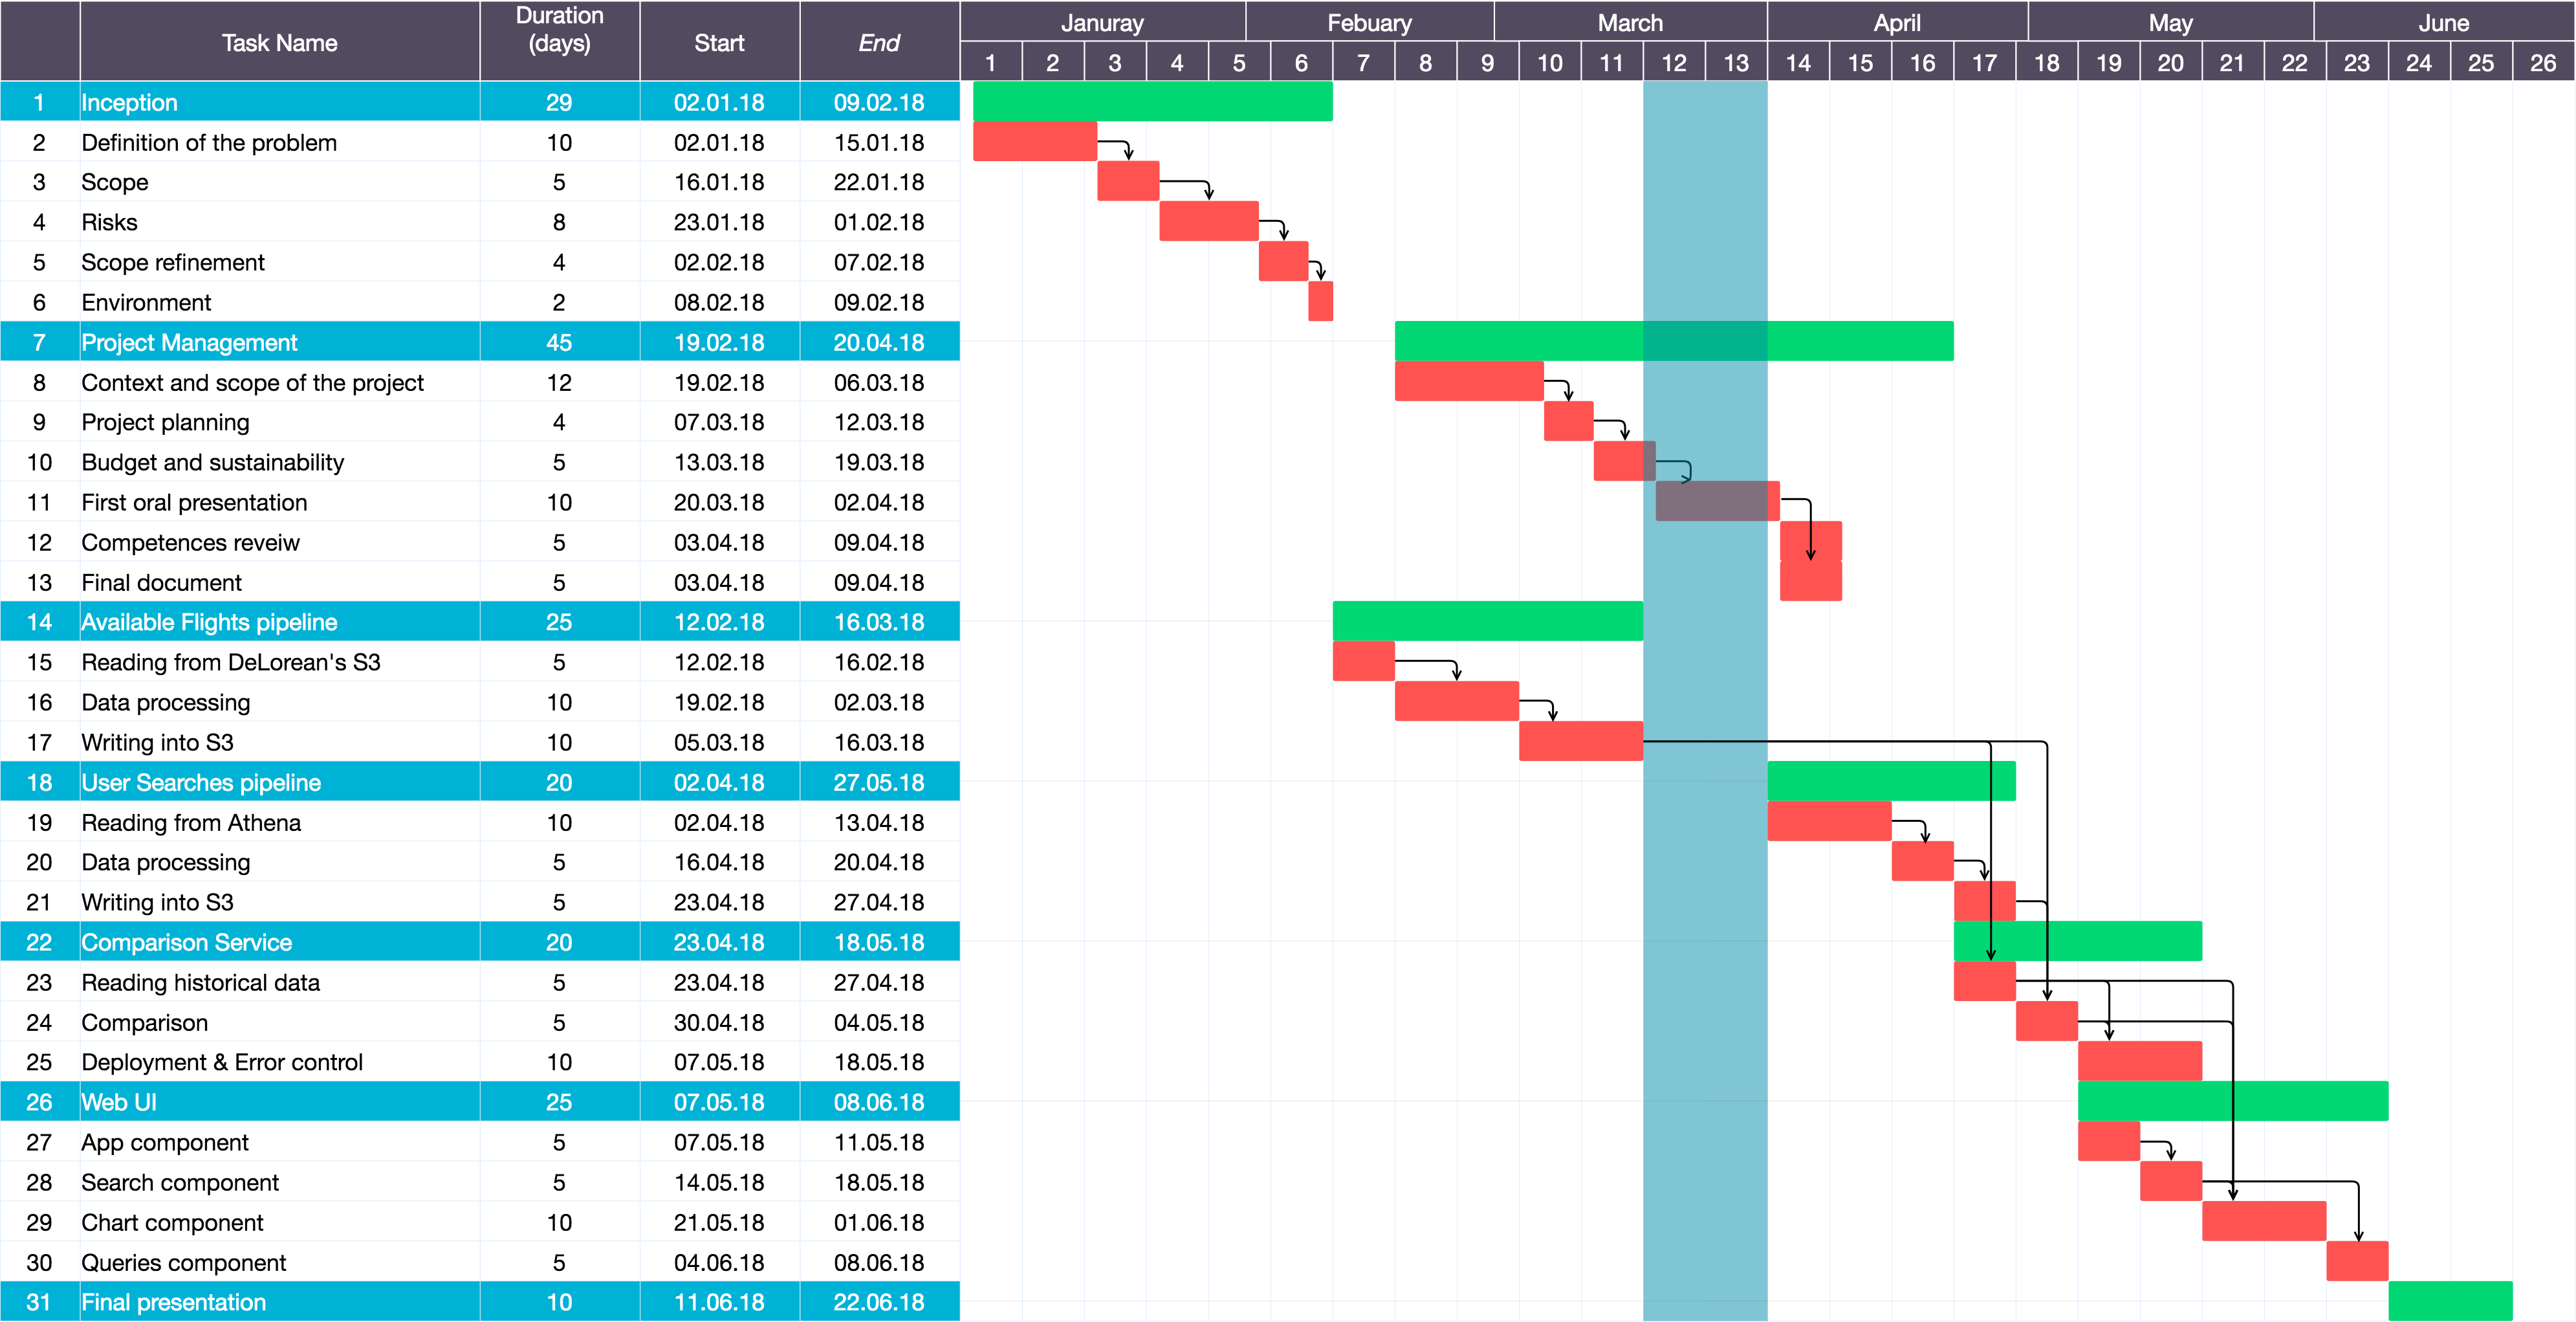
\includegraphics[scale=0.15,  angle =90]{diagrams/gantt.png}
\caption{Gantt diagram.}
\end{figure}



